% Chapter 3

\chapter{研究设计}
\section{数据}
\subsection{数据样本}
本文使用的公司财务报表数据和股票交易数据来自国泰安(CSMAR)数据库,因子模型数据分别来自中央财经大学金融学院、BetaPlus小组以及WHUFT异象因子数据集。由于我国A股上市公司的季报数据自2002年起才开始公布,为了保障数据的完整性,本文财务指标数据以2003年第一季度为数据的起点;而因子模型数据始于2003年10月。综上,本文数据样本时间区间为2003年12月至2020年9月,频次为季度。

对于股票样本的选择,本文以我国A股市场2018年底前上市的公司作为数据样本,规避未来收益数据的缺失。由于ST股票存在退市风险、金融行业公司财务报表结构有别于上市公司等原因,本文剔除掉ST股票、金融类股票,最后剩余3300支。有关数据缺失部分,若某支股票在第$t$期某一指标数据存在缺失,则剔除该股票在$t$期的所有数据。

在完成以上筛选步骤后,2003年12月至2020年9月的有效样本共119779条。图~\ref{size}~展示了 2003年12月至2020年9月季频月度有效样本量。总体来看,月度样本量随年份呈现上升趋势,由 2003年12月的872条有效样本增至2020年9月的2616条。

\begin{figure}[htbp]
  \centering
    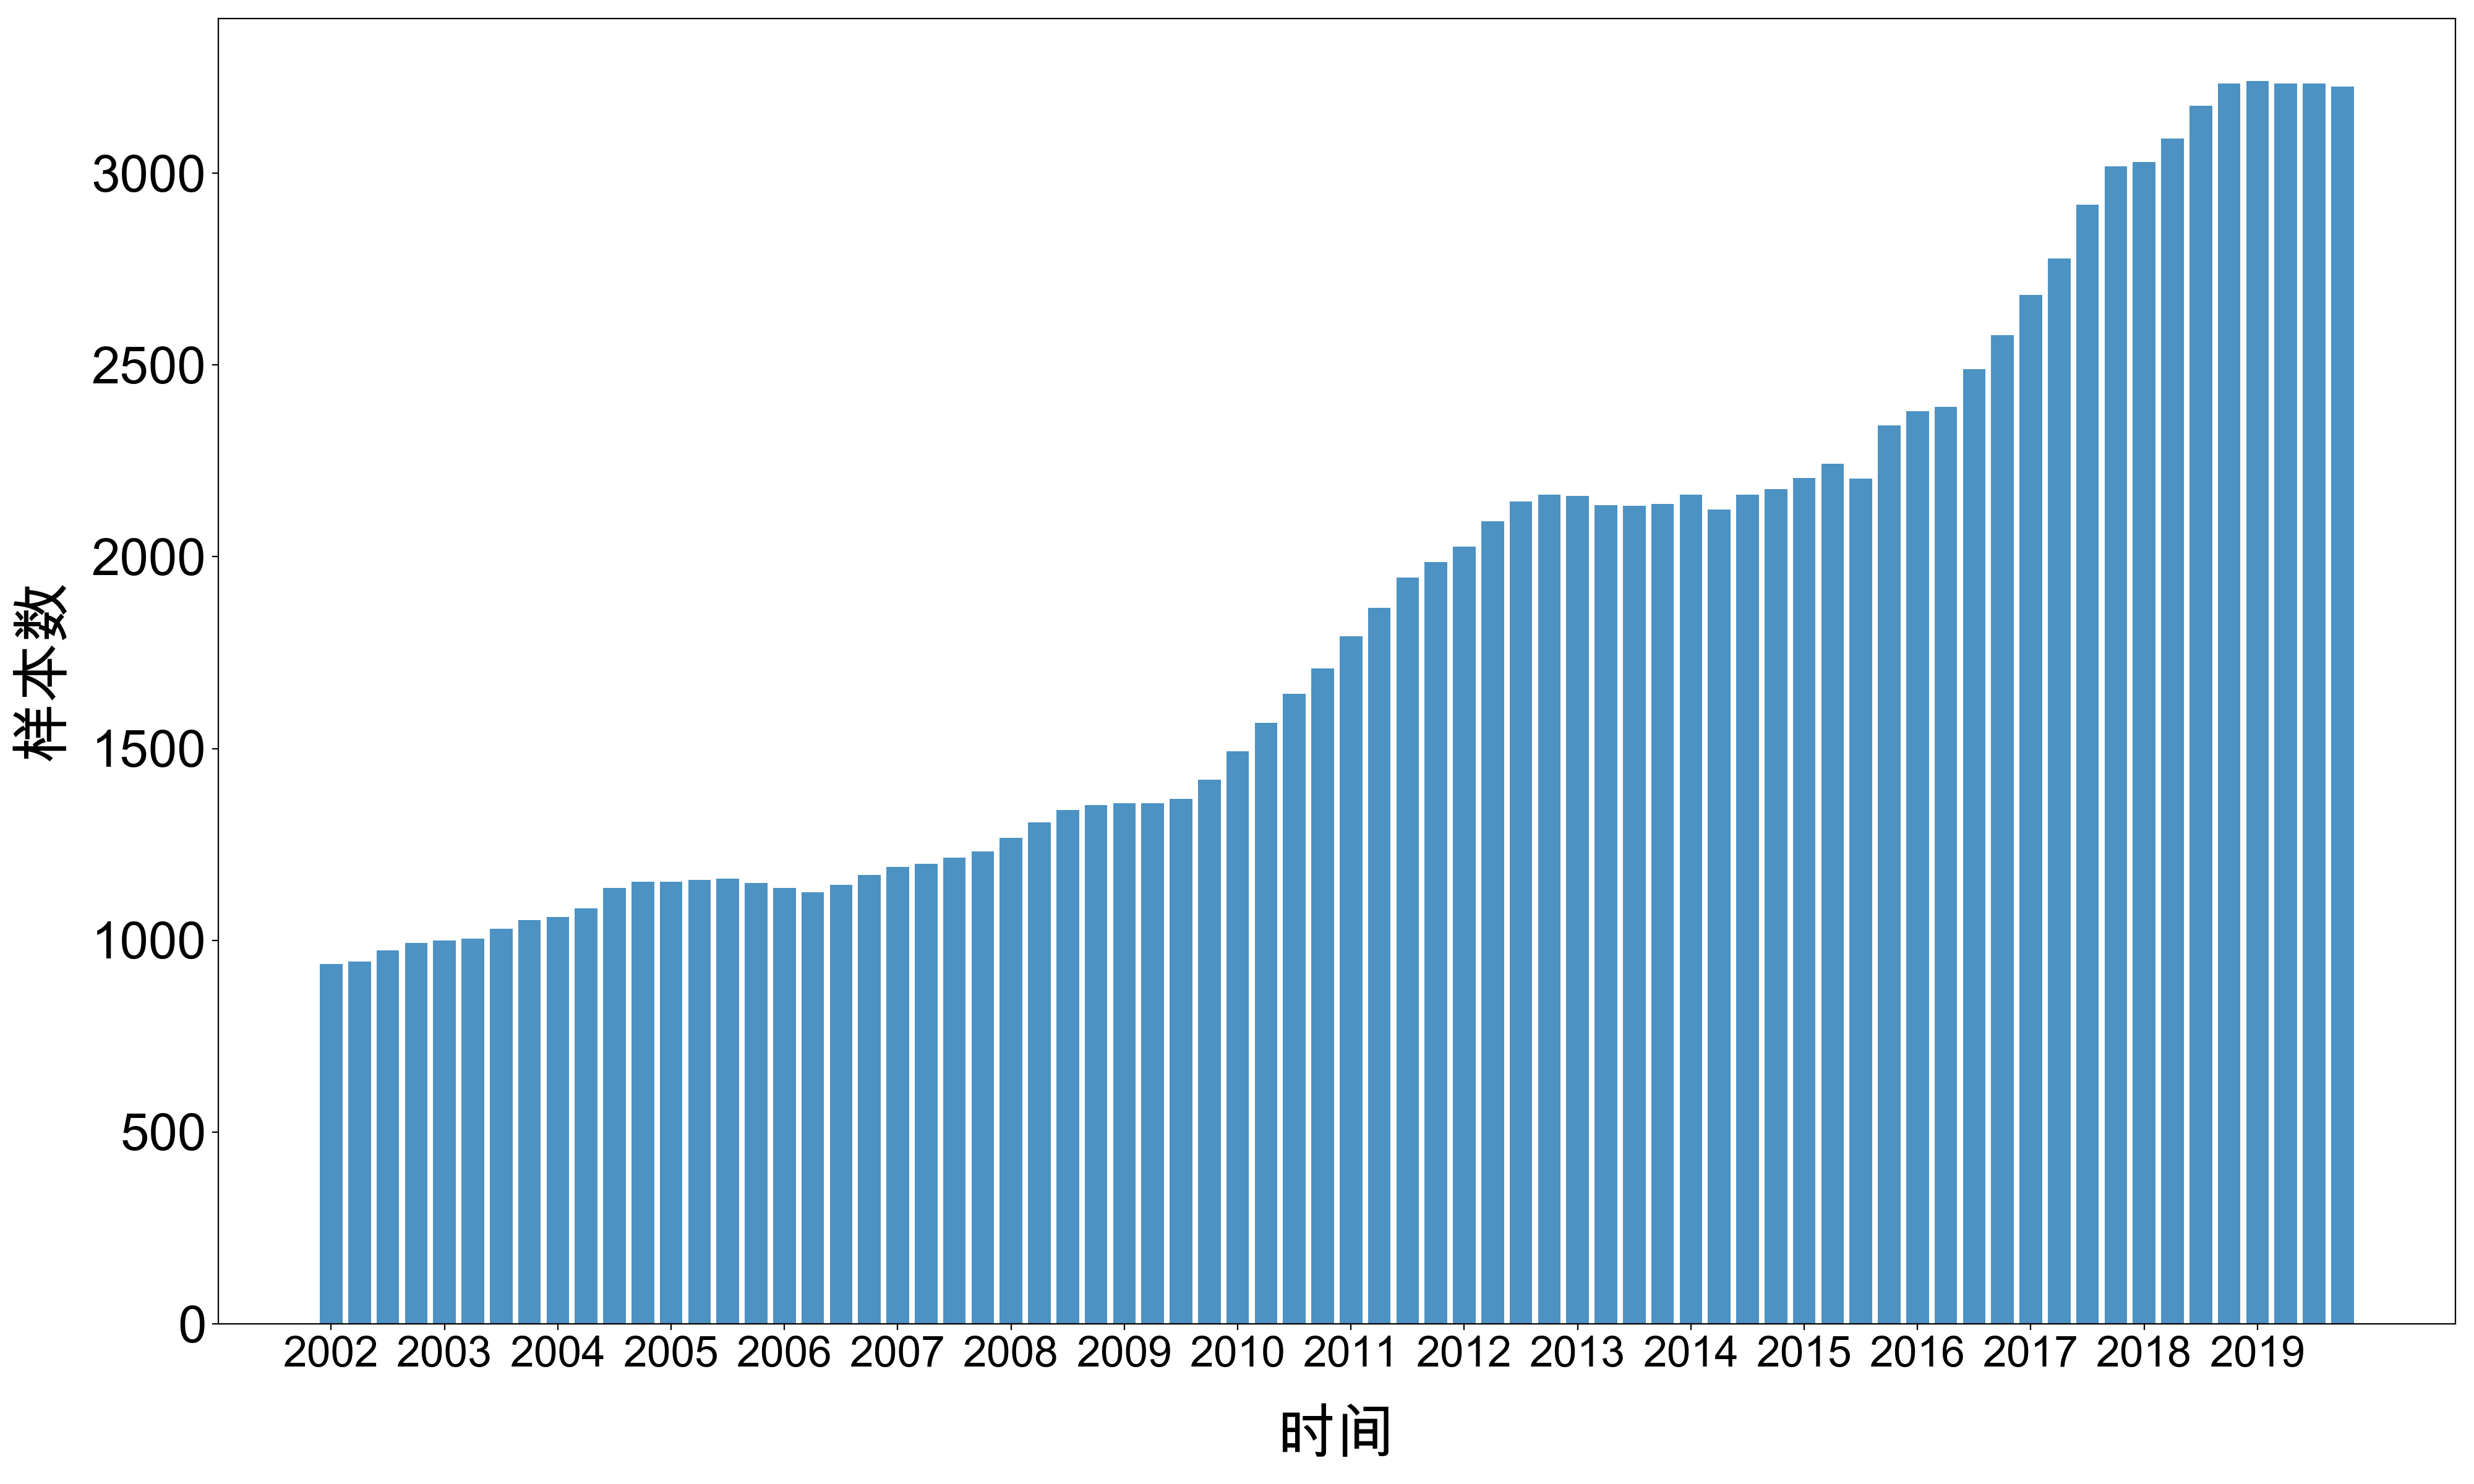
\includegraphics[width=\linewidth]{sample_size.png}
    \caption{样本数据的月度有效样本量}
    \label{size}
\end{figure}

\section{实证方法}
\subsection{变量定义与说明}
为了计算公司的错误定价因子M,首先需要对公司的内在价值进行估计。本文以公司市场价值为因变量,财务指标为自变量进行回归计算,得到的残差即为错误定价;之后通过Fama-MacBeth截面回归、因子模型回归等方法验证错误定价因子M的有效性。文章中采用的主要变量如表~\ref{variable}~所示:
\begin{table}[htbp]
  \centering
  \caption{变量定义与说明}
  \label{variable}
  \begin{tabular*}{0.9\hsize}{@{\hskip\tabcolsep\extracolsep\fill}*{2}{c}}
    \toprule
    变量名 & 定义及说明   \\
    \midrule
   $ mktcap_{it} $  & 公司$i$于季度$t$时的市场价值  \\
   $M_{i, t}$  & 公司$i$于季度$t$时的错误定价因子  \\
    $R_{i, t}$  &公司$i$于季度$t$时的月个股收益率  \\
    $BM$ & 市净率\\
    $beta $  & 市场投资组合$\beta$值 \\
    $grltnoa$ & 净经营性资产增长率\\
    $PA  $   & 毛利率\\
    $EP$   & 市盈率 \\
    $lagretn$ &上一个月的收益率\\
    $mom12$ &t-12月至t-2月的累计收益率(共计11个月) \\
    $mom36$ & t-36月至t-13月累计收益率(共计24个月)\\
          \bottomrule
  \end{tabular*}
\end{table}

\subsection{模型设定}
现有研究中,常见的公司内在价值计算方法包括现金流贴现法、相对价值法、经济附加值法、实物期权法等。这些方法虽然能起到一定的预测作用,但由于其选择的指标过少、过于死板,或太过于依赖使用者对未来的主观预测结果,亦或计算方法过于程式化等原因,很难排除掉数据窥视带来的影响。

根据本文的基本面分析原理,公司内在价值反映在一系列财务指标中,如式~\ref{eq1}~所示,其中$i$代表不同公司,$t$代表不同时间节点。$mktcap_{i, t}$ 为公司$i$于季度$t$时的市场价值,$f(.)$定义了一个参数为$\theta$的函数,在本文中为采用机器学习方法中的函数形式,$ I_{i, t}=( I_{i, t,1},I_{i, t,2},...,I_{i, t,N})$代表公司$i$在第$t$期时$N$个财务指标向量,$\epsilon_{i, t}$为残差项。本文将在后文中介绍采用的机器学习算法。
\begin{equation}
\label{eq1}
mktcap_{i, t} =f(I_{i, t};\theta)+\epsilon_{i, t} 
\end{equation}

对于财务指标的选择,为避免数据窥视的影响,并非由笔者主观挑选。相反,本文于CSMAR数据库下载了所有财务报表数据,包括资产负债表、利润表与直接法和间接法计算的现金流量表,共计262个指标。但由于不同公司个体财务情况差异大,过于细分的指标数据未被使用,或是数据库数据录入缺失等原因,为了计算的严谨性,将对262个财务指标进行筛选。

基于统计,在所有财务指标中,缺失值比例最大达到93.6\%,最小为0.01\%,均值高达41.6\%,说明有很多指标数据缺失情况严重,故选择缺失值比例小于等于5\%的所有指标,一共有51个。

在确定财务指标后,本文将采用随机森林(Random Forest,简称RF)和梯度提升树(Gradient Boosting Decision Tree,简称GBDT)方法进行数据模拟,确定具体函数形式$f(.)$。所有机器学习模型参数的选择均采用网格调参(Grid Search)的方式。由于本文需要逐期进行模型参数的选择,所以在获取每一期的最优参数后,进行式~\ref{eq1}~的回归,以确定该期的错误定价情况。
\begin{equation}
\label{eq2}
M_{i, t} =-1 \times \frac{\epsilon_{i, t}}{mktcap_{i, t}}
\end{equation}

回归后残差即为公司市值与内在价值的偏差,将该残差基于市值进行标准化后的负值,定义为错误定价因子M,如式~\ref{eq2}~所示。当公司内在价值低于市场价值时,即残差大于0,对应M为负值,说明股票被高估;当公司内在价值高于市场价值时,M为正值,说明股票被低估。

其中,考虑到市场以及公司的变化情况,公司的内在价值以及错误定价因子M每期都会重新计算一次,对公司进行重新分组调整,避免数据偏误。

总而言之,本文的统计方法不会偏好特定的股票市场、不考虑整个市场在给定时间点是否被高估或低估、也不依赖于内在价值的理论模型。相反,本文将公司进行相互比较,使用拟合优度的统计标准来识别公司内在价值如何体现于会计属性。

后续研究中,每期都将根据错误定价因子M大小进行公司分组:Q1到Q5五组。其中Q1为M最小的公司,即股票最被高估;Q5为M最大的公司,即股票最被低估。如果基本面分析有效、财务指标蕴含公司的内在价值,当市场价值最终趋近于内在价值时,最被高估的股票价格会回落,最被低估的股票价格会爬升,以此构建低买高卖的投资组合来获利。

为验证上述猜想,后文将进行Fama-MacBeth横截面回归、因子模型回归以及稳健性分析,如式~\ref{eq3}、\ref{eq4}~所示。
\begin{equation}
\label{eq3}
R_{i, t+1}=a_{t}+b_{t} M_{i, t}+\sum_{k=1}^{K} c_{k, t} X_{i, k, t}+\epsilon_{i, t+1}
\end{equation}
\begin{equation}
\label{eq4}
R_{i, t}=\alpha_{i}+\sum_{k=1}^{K} \beta_{i, k} F_{k, t}+\epsilon_{i, t}
\end{equation}

式~\ref{eq3}~中$X_{i, k, t}$代表公司$i$于季度$t$时第$k$个公司特征,作为控制变量,具体特征见表~\ref{variable}~所示;若$b_{t}$显著,说明错误定价因子M能够有效预测股票价格未来走势,证明了其有效性。

式~\ref{eq4}~中$F_{k,t}$为季度$t$时第$k$个因子值,本文主要采用Fama-French 三因子模型、Carhart 四因子模型、Fama-French 五因子模型、以及Hou-Xue-Zhang 四因子模型(后称为q-因子模型)进行分析;其中$\alpha_{i}$代表该投资组合的超额收益。如果Q1到Q5五组超额收益$\alpha$有显著的递增趋势,或是Q1、Q5的多空组合超额收益$\alpha$显著大于0,也能证明错误定价因子M的有效性。


\subsection{描述性统计}
表~\ref{description1}、\ref{description2}~列出了使用随机森林和GBDT两种方法计算的相关变量的描述性统计,这里将样本根据错误定价因子M分成了Q1到Q5五组进行考察。其中第一列为所有数据的平均值,第二列为错误定价因子M与相应变量的相关系数,第三列为Q1组(价值最被高估)的变量平均值,最后一列为Q5组(价值最被低估)的变量平均值。

%\setlength{\tabcolsep}{1.2mm}{
%\begin{table}[htbp]\centering
%\def\sym#1{\ifmmode^{#1}\else\(^{#1}\)\fi}
%\caption{描述性统计}
%\label{description}
%\begin{tabular*}{\hsize}{@{\hskip\tabcolsep\extracolsep\fill}*{8}{c}}
%\toprule
%               &\multicolumn{1}{c}{}&\multicolumn{1}{c}{}&\multicolumn{5}{c}{错误定价因子M分组}\\\cline{4-8} 
%          &\multicolumn{1}{c}{所有数据}&\multicolumn{1}{c}{相关系数}&\multicolumn{1}{c}{Q1 (被高估)}&\multicolumn{1}{c}{Q2}&\multicolumn{1}{c}{Q3}&\multicolumn{1}{c}{Q4}&\multicolumn{1}{c}{Q5 (被低估)}\\
%          &\multicolumn{1}{c}{(1)}&\multicolumn{1}{c}{(2)}&\multicolumn{1}{c}{(3)}&\multicolumn{1}{c}{(4)}&\multicolumn{1}{c}{(5)}&\multicolumn{1}{c}{(6)}&\multicolumn{1}{c}{(7)}\\
%\midrule
%$M $        &  -0.3821&1.000&  -1.0051&  -0.7446&  -0.5579&  -0.2682&   0.6674\\
%$mktcap$   &7.6048&0.007&8.2524&7.0417&6.6697&7.8798&8.1801\\
%$R_{t}$   &   0.7198&-0.051&   1.6784&   1.3812&   0.7776&   0.3141&  -0.5551\\
%$R_{t+1}$ &   0.7098&0.014&   0.5514&   0.6304&   0.6386&   0.7707&   0.9575\\
%$lagretn$  &   0.0316&-0.036&   0.0368&   0.0359&   0.0331&   0.0287&   0.0236\\
%$BM$        &   0.4457&0.283&   0.3201&   0.3597&   0.4343&   0.5023&   0.6195\\
%$EP$        &   0.0198& 0.017&  0.0147&   0.0183&   0.0214&   0.0219&   0.0228\\
%$beta $     &   1.1405&-0.005&   1.1321&   1.1461&   1.1509&   1.1420&   1.1309\\
%$grltnoa$   &   1.6139&-0.009&   5.3329&   1.5416&   0.3580&   0.2047&   0.2861\\
%$PA  $      &   0.0134&-0.048&   0.0133&   0.0145&   0.0147&   0.0135&   0.0106\\
%\bottomrule
%\end{tabular*}
%\end{table}}

\setlength{\tabcolsep}{1.2mm}{
\begin{table}[htbp]\centering
\def\sym#1{\ifmmode^{#1}\else\(^{#1}\)\fi}
\caption{描述性统计(随机森林方法)}
\label{description1}
\begin{tabular*}{\hsize}{@{\hskip\tabcolsep\extracolsep\fill}*{8}{c}}
\toprule
               &\multicolumn{1}{c}{}&\multicolumn{1}{c}{}&\multicolumn{5}{c}{错误定价因子M分组}\\\cline{4-8} 
          &\multicolumn{1}{c}{所有数据}&\multicolumn{1}{c}{相关系数}&\multicolumn{1}{c}{Q1 (被高估)}&\multicolumn{1}{c}{Q2}&\multicolumn{1}{c}{Q3}&\multicolumn{1}{c}{Q4}&\multicolumn{1}{c}{Q5 (被低估)}\\
          &\multicolumn{1}{c}{(1)}&\multicolumn{1}{c}{(2)}&\multicolumn{1}{c}{(3)}&\multicolumn{1}{c}{(4)}&\multicolumn{1}{c}{(5)}&\multicolumn{1}{c}{(6)}&\multicolumn{1}{c}{(7)}\\
\midrule
$M$       &   0.2215&    1.000&  -0.2709&  -0.0812&   0.0930&   0.3301&   1.0379\\
$mktcap $  & 7.9267&   -0.094&  13.9565&  11.2976&  7.4287&   4.4057&   2.5323\\
$R_{t}$   &   0.8405&   -0.083&   2.9935&   1.2586&   0.4508&  -0.0584&  -0.4461\\
$R_{t+1}$ &   0.7851&    0.039&   0.3790&   0.5373&   0.7598&   0.9499&   1.3007\\
$lagretn $  &   0.0316&   -0.035&  0.0485&   0.0319&   0.0280&   0.0245&   0.0251\\
$BM$    &  0.4498&    0.169&   0.2908&   0.4131&   0.4939&   0.5333&   0.5232\\
$EP  $      &  0.0207&    0.019&   0.0154&   0.0217&   0.0225&   0.0221&   0.0217\\
$beta$     &    1.1422 &    0.008&   1.1238&  1.1396&   1.1452&   1.1525&   1.1508\\
$grltnoa$ &     1.7915&   0.027&   0.3476&   0.2675&   0.4031&   0.2278&   8.4563\\
$PA$        &    0.0141 &  -0.027&   0.0175&   0.0152&   0.0126&   0.0116&   0.0134\\
\bottomrule
\end{tabular*}
\end{table}

\begin{table}[htbp]\centering
\def\sym#1{\ifmmode^{#1}\else\(^{#1}\)\fi}
\caption{描述性统计(GBDT方法)}
\label{description2}
\begin{tabular*}{\hsize}{@{\hskip\tabcolsep\extracolsep\fill}*{8}{c}}
\toprule
               &\multicolumn{1}{c}{}&\multicolumn{1}{c}{}&\multicolumn{5}{c}{错误定价因子M分组}\\\cline{4-8} 
          &\multicolumn{1}{c}{所有数据}&\multicolumn{1}{c}{相关系数}&\multicolumn{1}{c}{Q1 (被高估)}&\multicolumn{1}{c}{Q2}&\multicolumn{1}{c}{Q3}&\multicolumn{1}{c}{Q4}&\multicolumn{1}{c}{Q5 (被低估)}\\
          &\multicolumn{1}{c}{(1)}&\multicolumn{1}{c}{(2)}&\multicolumn{1}{c}{(3)}&\multicolumn{1}{c}{(4)}&\multicolumn{1}{c}{(5)}&\multicolumn{1}{c}{(6)}&\multicolumn{1}{c}{(7)}\\
\midrule
$M$       &    0.2950& 1.000& -0.3103&  -0.0609&   0.1415&   0.4320&   1.2745\\
$mktcap $  & 7.9267 &  -0.090&  9.6631&  14.5515&  10.1442&   3.4469&   1.8191\\
$R_{t}$   &    0.8405& -0.094&   2.8204&   1.2833&   0.5060&   0.0062&  -0.4172\\
$R_{t+1}$ &   0.7851&  0.036&  0.2922&   0.5722&   0.7975&   0.9624&   1.3025\\
$lagretn $  & 0.0316&   -0.030&   0.0464&   0.0303&   0.0248&   0.0261&   0.0304\\
$BM$    &   0.4498&    0.094&   0.3057&   0.4464&   0.5233&   0.5142&   0.4614\\
$EP  $      &  0.0207 &   -0.043&   0.0158&   0.0238&   0.0256&   0.0204&   0.0176\\
$beta$     &  1.1422&   -0.005&   1.1293&   1.1331&   1.1364&   1.1523&   1.1619\\
$grltnoa$ &   1.7915&    0.008&   0.3489&   0.4555&   0.1699&   2.4593&   6.3972\\
$PA$        & 0.0141&   -0.058&   0.0172&   0.0155&   0.0137&   0.0111&   0.0128\\
\bottomrule
\end{tabular*}
\end{table}
}

在两个描述性统计表格中,从第三列到最后一列,第$t-1$期到第$t$期的收益$R_t$逐渐减少,说明购买被高估的股票收益更高,与现实情况相符,同时第$t$期前一个月的收益lagretn也是逐渐减少的趋势。但是,第$t$期到第$t+1$期的收益$R_{t+1}$逐渐增加,说明被高估的股票价格下降,逐渐趋于正常,所以收益变低,而被低估的股票价值上涨到正常价值,收益变高,与本文猜想保持一致。

相比于被高估的Q1组股票,被低估的Q5组股票平均有着更高的市净率BM与市盈率EP,同样有着更低的市场价值mktcap;再加上错误定价因子M与市净率BM有着正相关关系,说明被高估的股票更多是高市值的价值股,而被低估的股票多是低市值的成长股。

错误定价因子M与beta相关系数低,说明系统性风险并不能解释M对于股票未来收益的预测能力。由于M与其他异象的相关系数基本都低于0.05,在后续回归中,将beta值、过去一个月的收益lagretn、市净率BM、市盈率EP、净经营性资产增长率grltnoa以及毛利率PA作为公司层面的控制变量。由于公司市值mktcap与错误定价因子M高度相关,在后续回归中为避免多重共线性问题,控制变量将不包含公司市值mktcap。


%\section{脚注}
%注释是对论文中特定名词或新名词的注解。注释可用页末注或篇末注的一种。选择页末注的应在注释与正文之间加细线分隔,线宽度为 1 点,线的长度不应超过纸张的三分之一宽度。同一页类列出多个注释的,应根据注释的先后顺序编排序号。字体为宋体5号,注释序号以“\circled{1}、\circled{2}”等数字形式标示在被注释词条的右上角。页末或篇末注释条目的序号应按照“\circled{1}、\circled{2}”等数字形式与被注释词条保持一致,脚注序号每面更新。示例:这里有个注释\footnote{我是解释注释的}。
%
%\section{引用文中小节}\label{sec:ref}
%如引用小节~\ref{sec:ref}
%
%\section{引用参考文献}
%这是一个参考文献引用的范例:“\cite{江泽民1989能源发展趋势及主要节能措施}提出……”。还可以引用多个文献:“\cite{kuhn2004man,江泽民2008新时期我国信息技术产业的发展,江泽民1989能源发展趋势及主要节能措施}提出……”。不同的引用方法:“\citet{江泽民1989能源发展趋势及主要节能措施}”“\citep{江泽民2008新时期我国信息技术产业的发展}”更多引用命令请参阅 natbib 文档或 biblatex 文档。\nocite{*}
%
%文献引用需要配合 BibTeX 使用,很多工具可以直接生成 BibTeX 文件(如 EndNote、NoteExpress、百度学术、谷歌学术等),此处不作介绍。
%
%\section{链接相关}
%模板使用了 hyperref 包处理相关链接,使用 \verb|\href| 可以生成超链接,默认不显示链接颜色。如果需要输出网址,可以使用 \verb|\url| 命令,示例:\url{https://github.com}。